% Note that if you want something in single space you can go back and
% forth between single space and normal space by the use of \ssp and
% \nsp.  If you want doublespacing you can use \dsp.  \nsp is normally
% 1.5 spacing unless you use the doublespace option (or savepaper
% option)
%
%(FORMAT) usually you *don't* want to mess with the spacing for your
%(FORMAT) final version.  If you think/know that the thesis template
%(FORMAT) and/or thesis style file is incorrect/incomplete, PLEASE
%(FORMAT) contact the maintainer.  THANK YOU!!!

\chapter{LINE SEGMENT INTERSECTION}
\label{chap:linesegintersec}
% By labeling the chapter, I can refer to it later using the
% label. (\ref{chap:linesegintersec}, \pageref{chap:linesegintersec}) Latex will take care
% of the numbering.

\section{Problem Definition}

Consider the example given in the previous chapter to find the intersections between roads and rivers in order to find the locations where bridges need to be built in the city. This problem is commonly known as the map overlay problem where the map of roads and rivers are superimposed upon each other. Roads and rivers are represented by lines and we need to find the intersection points among those lines or the region induced by those line intersections. We are going to consider an efficiency-minded modification of the algorithm for the simple case of finding the intersection points among line segments as the scope of this thesis. Let�s describe the problem geometrically first. Consider the rivers as one set of line segments and roads as another set of segments. We then need to find the point of intersection between these two sets of segments. However, the problem specification is not yet precise enough. We have not specified what to do in various degenerate cases, such as when two line segments intersect because their endpoints meet at a common point.  We could require two line segments always to intersect only in the interior of the lines.  This essentially becomes the question of whether the two line segments are open or closed. As with the representation of curved features in a map, we will make some assumptions that simplify the approach. Later we shall realize that it is easy to consider these special cases without changing the basic nature of the algorithm. We will assume the line segments to be such that they are open (we do not have to worry about endpoint-only intersections--said another way, we will consider the point as an intersection point even if it happens to be on the end of the line segment) and no more than two line segments intersect at a single point (we do not have to worry about multiple intersections in the same place). Furthermore, none of the line segments are parallel to each other. 

For the sake of simplicity and without loss of generality, we will consider the line segments from two different sets (e.g. rivers and roads) to be members of a single set. We will compute the intersection among all the lines in this single set. We will obviously get some intersection points among the same set of line segments when we merge these two sets together, and we can remove this ambiguity later. To do this we simply store the original segments involved so that at the end we can discard the intersection points which belong to segments from the same original set. Thus the required intersection points can be filtered out easily. Storing of these line segments along with the intersection points may seem like a bit of storage overhead at first glance but most of times it is often required in other places too. Let�s say that we want to consider the intersection points among line segments based on the spatial extent. In that case we would need the information about the intersecting line segments in order to filter them out based on the spatial extent. Finally we will state our problem specification as follows: given a set S of n closed segments in the plane (Figure.~\ref{fig3} \cite{TEXTBOOK}), report all intersection points among the segments in S.
\begin{figure}[ht]
  \begin{center}
   	\fbox{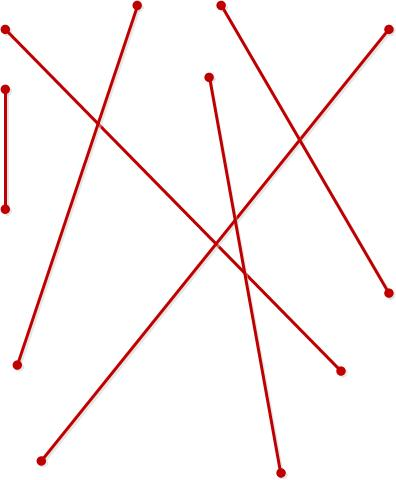
\includegraphics[width=3in, height=2.5in]{Figures/Figure3}}
  \end{center}
  \centering
	\parbox{3in}{\caption{Segments in a 2-dimensional space. Adapted from Source : M. DE BERG, M. VAN KREVELD, M. OVERMARS, AND O. SCHWARZKOPF,
\textbf{\textit{Computational Geometry- Algorithms and Applications}}, Springer Verlag, Berlin, Germany, 2000, ch. 2, pp. 19-29.} \label{fig3}} 
\end{figure}

\section{Potential Solution}

This may seem like an easy problem at first glance where we simply need to take each line segment and perform intersection tests with each of the other line segments. This algorithm would require O(n2) time. Unfortunately this would actually be the optimal solution in the case where all the line segments in a set intersect with every other line segment in the other set. This is called an output-bound problem. We may find an efficient algorithm in general, but certain so-called pathological cases can cause its running time to degenerate into this worst-case quadratic performance. In practical situations, however, most segments intersect none or only a few of the other segments. Thus the total number of intersection points is quite less and seldom leads to this quadratic performance. As we will see, the algorithm is as efficient as possible (that is, it is optimal) except in these rare cases. 

\section{Draft of the Algorithm}

How could we avoid testing all the pairs of line segments for intersection in order to improve the asymptotic time (in the general, non-pathological arrangement)? We can make use of the geometry of the situation and perform intersection tests only of the segments that are close to each other at some point in our algorithm. This is based on the geometric insight that segments must become close to each other to intersect. How do we find out which line segments are close to each other? What do we exactly mean by being close to each other (for example horizontally or vertically or along some other direction)?

Let L := {La, Lb, �, Ln} be the set of segments for which we want to compute all the intersections. Now we need to find out which segments among these are close to each other. Consider the y-interval of these line segments to be its orthogonal projection onto y-axis (Figure.~\ref{fig4} \cite{TEXTBOOK}). Now when the y-interval of two or more segments overlaps then these segments are considered close to each other and we can perform intersection tests on them. The line segments whose y-interval does not overlap are far apart in the y direction and cannot intersect with each other. Thus we only need to test the pair of segments whose y-intervals overlap with each other. In other words, we need to test the pair of segments for which there exists a horizontal line that intersects both the segments, given that no other segments, besides the two in the pair, are intersected by the horizontal line at any point between the intersections between it and the pair. To be more precise about finding these pairs, consider an imaginary line �S� sweeping downwards over the plane starting at a position above all the line segments. We can keep track of the line segments intersecting this sweeping line as it moves downwards.

This algorithmic technique is called the line-sweep (or sometimes plane-sweep) algorithm and the line �S� is called the sweep line. The data structure that maintains information about the set of lines segments intersecting the sweep line at any given point is called the status of the sweep line. This data structure, called the status structure, is typically implemented as a kind of balanced binary search tree. The status changes as the sweep line moves downwards but it does not need to be updated continuously. The status structure is updated only at certain points called event points. These event points are the end points of the line segments, as well as intersection points that are discovered along the way (Figure.~\ref{fig5} \cite{TEXTBOOK}).
\begin{figure}[ht]
  \begin{center}
   	\fbox{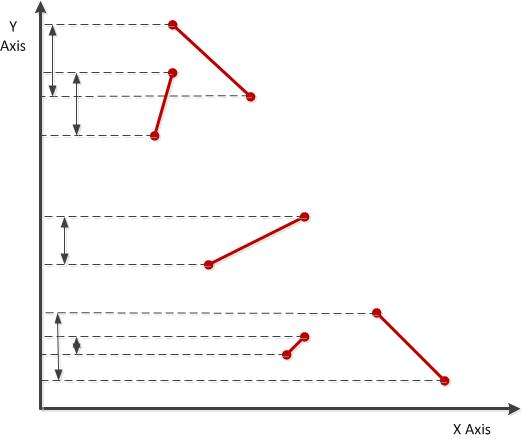
\includegraphics[width=3.5in, height=3.5in]{Figures/Figure4}}
  \end{center}
  \centering
	\parbox{3.5in}{\caption{Lines showing their orthogonal projection onto Y axis. Adapted from Source: M. DE BERG, M. VAN KREVELD, M. OVERMARS, AND O. SCHWARZKOPF, \textbf{\textit{Computational Geometry- Algorithms and Applications}}, Springer Verlag, Berlin, Germany, 2000, ch. 2, pp. 19-29.} \label{fig4}} 
\end{figure}

When the sweep line reaches these end points, it is only then that the status structure is updated and the algorithm actually does something. When the sweep line reaches the upper end point of a line segment, then a new segment starts intersecting the sweep line and intersection test is performed against all the line segments adjacent to each other along the sweep line at that point. If the end point is the lower end point of the line segment then that segments stops intersecting the sweep line and that line segment can be deleted from the status structure (the sweep line will never again encounter it). This is how we only perform the intersection tests on segments that are �close� or  adjacent, i.e. for which the horizontal line passes through them in succession, excluding all other pairs and thereby affording us the avoidance of the quadratic check of every pair and improving the efficiency of the algorithm.
\begin{figure}[ht]
  \begin{center}
   	\fbox{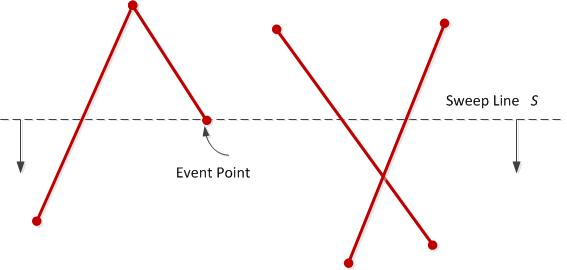
\includegraphics[width=6in, height=3in]{Figures/Figure5}}
  \end{center}
  \centering
	\parbox{6in}{\caption{Event point of a line. Adapted from Source: M. DE BERG, M. VAN KREVELD, M. OVERMARS, AND O. SCHWARZKOPF, \textbf{\textit{Computational Geometry- Algorithms and Applications}}, Springer Verlag, Berlin, Germany, 2000, ch. 2, pp. 19-29.} \label{fig5}} 
\end{figure}

\section{Some Problems and their Solutions}

Unfortunately this approach can fail in certain conditions. We can still end up performing intersection tests on a quadratic number of pairs even though there may actually be substantially fewer intersections. A simple example can be where we have a number of vertical lines that intersect x-axis. The problem is that the two segments that intersect the sweep line can still be far apart in the horizontal direction even though they are closer in the y direction.

To solve this problem, let us order the line segments from left to right. Now we will perform intersection tests only on the segments that are adjacent to each other so that we test only the segments that close to each other in the horizontal direction. Thus each line segment is tested for intersection with two adjacent line segments, namely, one to left and other to the right of it. This comparison is made based on the upper end point. The status should now correspond to this new strategy reflecting the ordered sequence of segments intersecting the sweep line. Thus the new status now not only changes at the end points of the line segments but it also changes at the intersection points which are computed at runtime on the fly. When a sweep line intersects an intersection point (Figure.~\ref{fig6} \cite{TEXTBOOK}), we must test the two segments for intersection against their new neighbors. This is a new type of event point besides the regular upper and lower end points of line segments.
\begin{figure}[ht]
  \begin{center}
   	\fbox{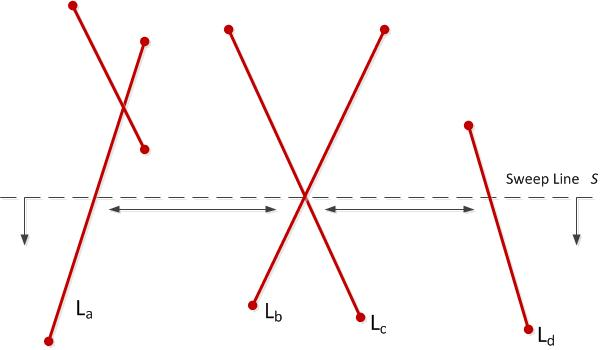
\includegraphics[width=5in, height=1.75in]{Figures/Figure6}}
  \end{center}
  \centering
	\parbox{5in}{\caption{Lines have new neighbors. Adapted from Source: M. DE BERG, M. VAN KREVELD, M. OVERMARS, AND O. SCHWARZKOPF, \textbf{\textit{Computational Geometry- Algorithms and Applications}}, Springer Verlag, Berlin, Germany, 2000, ch. 2, pp. 19-29.} \label{fig6}} 
\end{figure}

Let�s discuss the approach we have discussed until now. Imagine there are n number of line segments in a two dimensional space. Now imagine a sweep line �S� that starts sweeping all the line segments. Initially the sweep line is placed above all the line segments. The sweep line maintains a status structure that indicates all the ordered line segments from left to right that intersect the sweep line at any particular instance of time. This status structure is updated at certain points called as event points. These event points are namely upper end point of a line segment, lower end point of a line segment and the intersection point of line segments that are detected at runtime (Figure.~\ref{fig8} \cite{TEXTBOOK}). We have to take several actions depending upon the type of event point.
\begin{figure}[ht]
  \begin{center}
   	\fbox{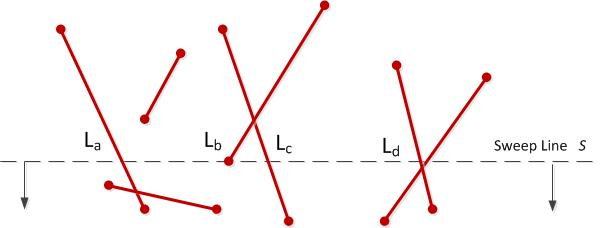
\includegraphics[width=5in, height=2in]{Figures/Figure8}}
  \end{center}
  \centering
	\parbox{5in}{\caption{Sweep line progressing through lines. Adapted from Source: M. DE BERG, M. VAN KREVELD, M. OVERMARS, AND O. SCHWARZKOPF, \textbf{\textit{Computational Geometry- Algorithms and Applications}}, Springer Verlag, Berlin, Germany, 2000, ch. 2, pp. 19-29.} \label{fig8}} 
\end{figure}

When the event point is an upper end point of a line segment then the sweep line starts intersecting a new line segment. This line segment must be inserted at appropriate position in the status structure and an intersection test must be performed against its two neighbors namely one to left and the other to the right side of it. When the event point is a lower end point of a line segment then the sweep line has reached the bottom of that line segment and hence will stop intersecting it. It must be deleted from the status structure and its neighbors must be considered for intersection as they now become new neighbors of each other. 

When the event point is an intersection point (Figure.~\ref{fig9} \cite{TEXTBOOK}) the two segments that intersect each other change their order along the sweep line. Each of them gets (at most) one new neighbor, against which they are tested for intersection. At each event point only the intersection point found below the sweep line are taken into consideration since those that are above the sweep line have already been detected and processed (Figure.~\ref{fig7} \cite{TEXTBOOK}). When all the event points are processed, then algorithm indicates that we have swept the plane all the way to the bottom and detected all the event points.
\begin{figure}[ht]
  \begin{center}
   	\fbox{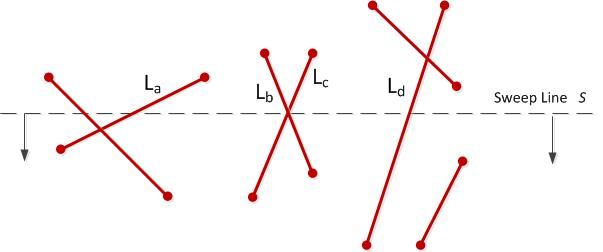
\includegraphics[width=6in, height=3in]{Figures/Figure9}}
  \end{center}
  \centering
	\parbox{6in}{\caption{Sweep line reaching an intersection point. Adapted from Source: M. DE BERG, M. VAN KREVELD, M. OVERMARS, AND O. SCHWARZKOPF, \textbf{\textit{Computational Geometry- Algorithms and Applications}}, Springer Verlag, Berlin, Germany, 2000, ch. 2, pp. 19-29.} \label{fig9}} 
\end{figure}
\begin{figure}[ht]
  \begin{center}
   	\fbox{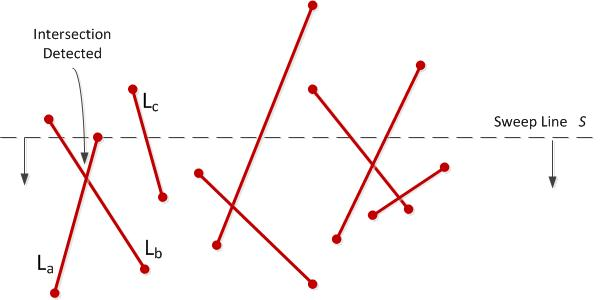
\includegraphics[width=6in, height=3in]{Figures/Figure7}}
  \end{center}
  \centering
	\parbox{6in}{\caption{Snapshot when an intersection point is detected. Adapted from Source: M. DE BERG, M. VAN KREVELD, M. OVERMARS, AND O. SCHWARZKOPF, \textbf{\textit{Computational Geometry- Algorithms and Applications}}, Springer Verlag, Berlin, Germany, 2000, ch. 2, pp. 19-29.} \label{fig7}} 
\end{figure}
